\section{Database design}\label{sec:database_design}

The primary database used for this project is a PostgreSQL database, hosted on Amazon RDS.
PostgreSQL is a powerful, open-source relational database management system that provides robust features for data storage, retrieval, and management.
It is chosen for its reliability, scalability, and support for extensive data types and extensions, making it suitable for handling the requirements of this project.

\subsection{Database schema}\label{subsec:database_schema}

The database schema was designed to cover the requirements of each of the phases of the data pipeline outlined in the system design.
The schema consists of several tables, each serving a specific purpose in the data pipeline.

The main tables in the database schema are as follows, and the schema diagram is shown in figure~\ref{fig:database_schema}:
\begin{itemize}
    \item \textbf{crawler\_pages:} This table stores the metadata associated with each crawled (or to be crawled) page.
    This table it primarily used to keep track of the crawling process, and is used to populate the crawler queue.
    In the later stages of the pipeline, it used to identify recently crawled pages to be passed to the page classification and information extraction modules.
    \item \textbf{minimized\_pages}: This table keeps track of the metadata associated with the page minimization phase.
    Similar to the \texttt{crawler\_pages} table, it is used to keep track of the minimization process and identify recently minimized pages to be passed to the page classification and information extraction modules.
    \item \textbf{page\_classifications}: This table stores the current results of the page classification phase, including the classification of each page as a product page or non-product page.
    \item \textbf{product\_information}: This table stores the extracted product information from the product pages, including the product name, price, image, and stock status.
    \item \textbf{price\_history}: This table stores the historical price data for each product, allowing for analysis of price trends and identification of genuine sales and discounts.
    This table is linked to the \texttt{product\_information} table via Change Data Capture (CDC) to ensure that any changes to the price in \texttt{product\_information} table are reflected in the \texttt{price\_history}.
    \item \textbf{product\_embeddings}: This table stores the embeddings of the product pages, which are used for product matching across different websites.
    The embeddings are generated using a pre-trained model and are stored in this table for efficient retrieval and comparison.
\end{itemize}

\begin{figure}[h]
    \centering
    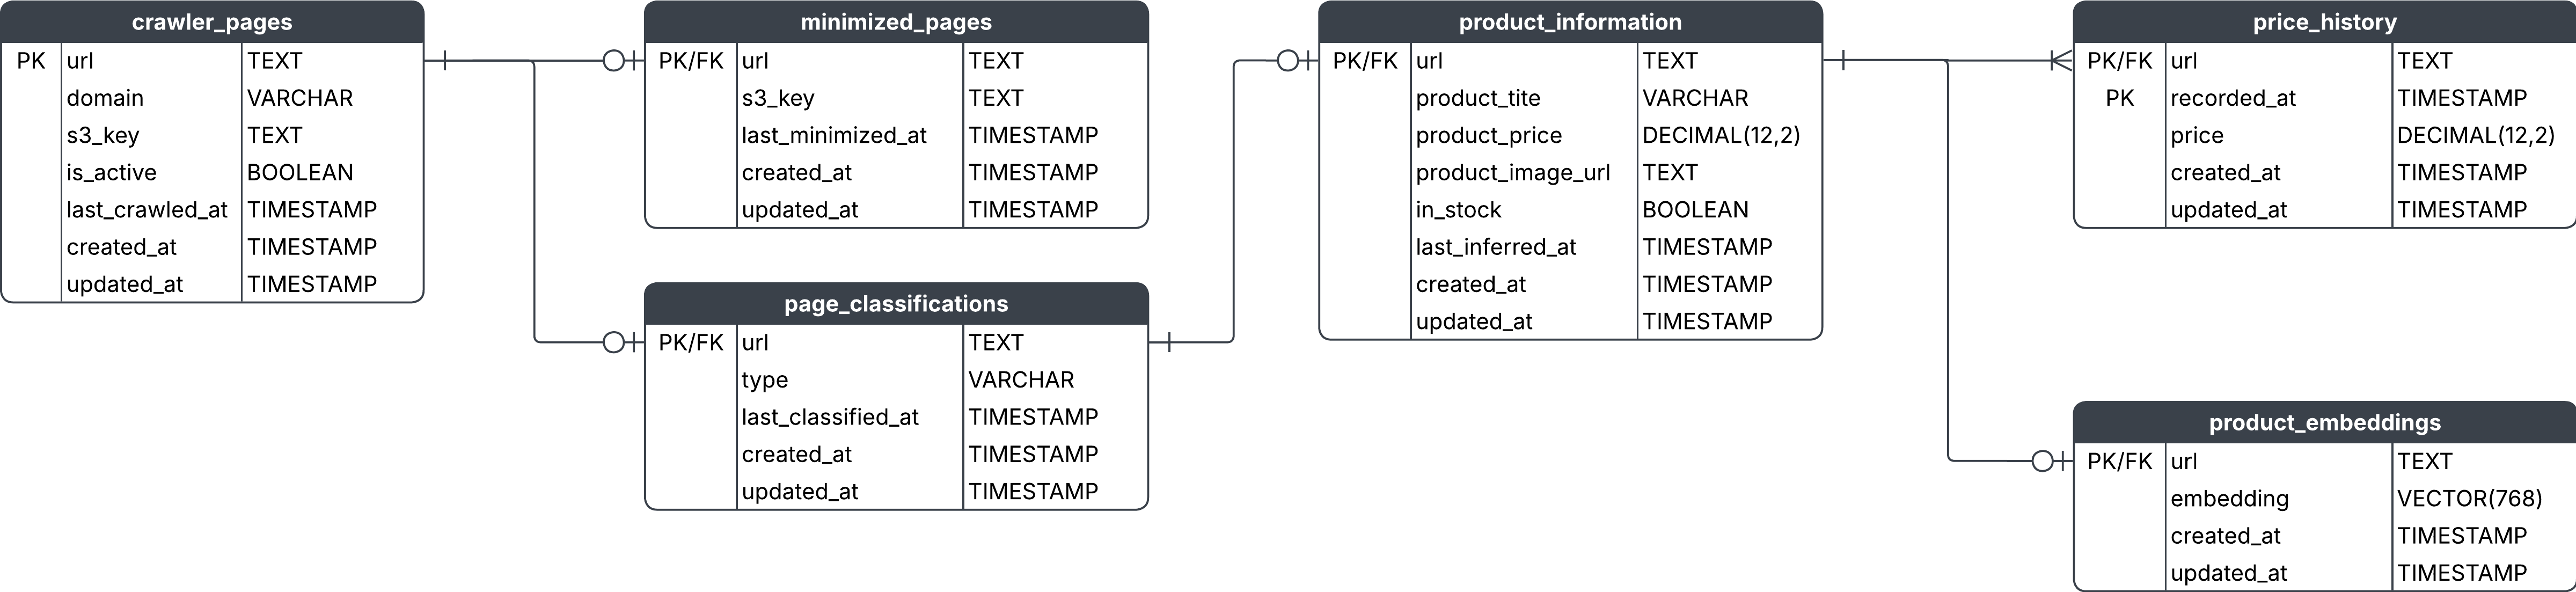
\includegraphics[width=\textwidth]{images/db_primary_schema}~\caption{Database schema diagram}\label{fig:database_schema}
\end{figure}

Aside from the main tables, there are two auxiliary tables which are only used for the model training phases, and are not connected to the components in the system or the other tables in the database schema.
These tables are as follows and their schema diagram is shown in figure~\ref{fig:database_auxiliary_schema}:

\begin{itemize}
    \item \textbf{page\_labels}: This table stored the annotated labels for the crawled pages, which are used for training the page classification model as well as the information extraction model.
    \item \textbf{matching\_products}: This table consists of pairs of matching and non-matching products, which are used for training the product matching embedding model.
\end{itemize}

\begin{figure}[h]
    \centering
    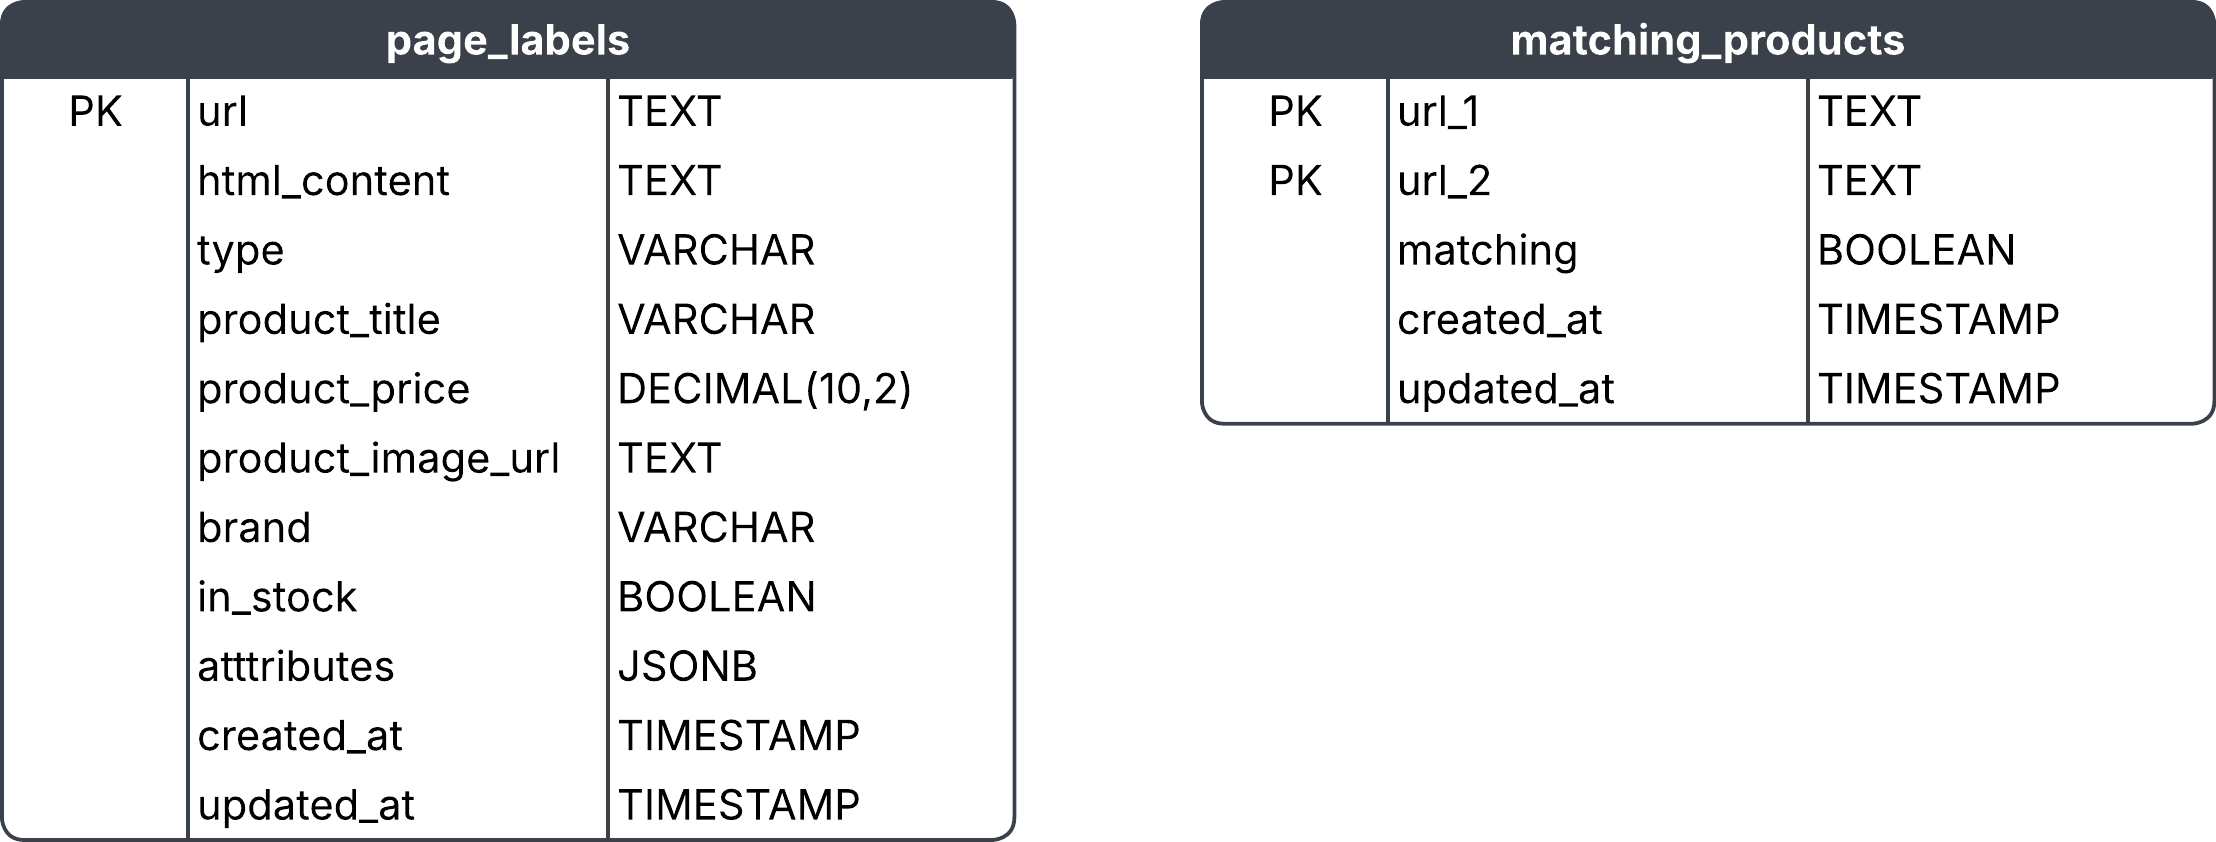
\includegraphics[width=0.6\textwidth]{images/db_auxiliary_schema}~\caption{Database auxiliary schema diagram}\label{fig:database_auxiliary_schema}
\end{figure}